%8 pages
%%
%% This is file `sample-sigconf.tex',
%% generated with the docstrip utility.
%%
%% The original source files were:
%%
%% samples.dtx  (with options: `sigconf')
%% 
%% IMPORTANT NOTICE:
%% 
%% For the copyright see the source file.
%% 
%% Any modified versions of this file must be renamed
%% with new filenames distinct from sample-sigconf.tex.
%% 
%% For distribution of the original source see the terms
%% for copying and modification in the file samples.dtx.
%% 
%% This generated file may be distributed as long as the
%% original source files, as listed above, are part of the
%% same distribution. (The sources need not necessarily be
%% in the same archive or directory.)
%%
%% The first command in your LaTeX source must be the \documentclass command.
\documentclass[sigconf,table]{acmart}

\usepackage{algpseudocode}
\usepackage{algorithm}
\usepackage{algorithmicx}
\usepackage{verbatim}
\usepackage{mathtools}
\usepackage{multirow}
\usepackage{subcaption}
\usepackage{colortbl}

\usepackage{tikz}
\usetikzlibrary{automata,positioning}

\definecolor{lightgray}{gray}{0.9}


%\def\BibTeX{{\rm B\kern-.05em{\sc i\kern-.025em b}\kern-.08em
	%	T\kern-.1667em\lower.7ex\hbox{E}\kern-.125emX}}

\usepackage{booktabs} % For formal tables


\newlength\Origarrayrulewidth

% horizontal rule equivalent to \cline but with 2pt width
\newcommand{\Cline}[1]{%
	\noalign{\global\setlength\Origarrayrulewidth{\arrayrulewidth}}%
	\noalign{\global\setlength\arrayrulewidth{3pt}}\cline{#1}%
	\noalign{\global\setlength\arrayrulewidth{\Origarrayrulewidth}}%
}

% draw a vertical rule of width 2pt on both sides of a cell
\newcommand\Thickvrule[1]{%
	\multicolumn{1}{!{\vrule width 2pt}c!{\vrule width 2pt}}{#1}%
}

% draw a vertical rule of width 2pt on the left side of a cell
\newcommand\Thickvrulel[1]{%
	\multicolumn{1}{!{\vrule width 2pt}c}{#1}%
}

% draw a vertical rule of width 2pt on the right side of a cell
\newcommand\Thickvruler[1]{%
	\multicolumn{1}{c!{\vrule width 2pt}}{#1}%
}

%%
%% \BibTeX command to typeset BibTeX logo in the docs
\AtBeginDocument{%
	\providecommand\BibTeX{{%
			\normalfont B\kern-0.5em{\scshape i\kern-0.25em b}\kern-0.8em\TeX}}}

%% Rights management information.  This information is sent to you
%% when you complete the rights form.  These commands have SAMPLE
%% values in them; it is your responsibility as an author to replace
%% the commands and values with those provided to you when you
%% complete the rights form.
\setcopyright{acmcopyright}
\copyrightyear{2020}
\acmYear{2020}
\acmConference[GRADES-NDA'20]{Joint Workshop on Graph Data Management Experiences \& Systems (GRADES) and Network Data Analytics (NDA)}{June 14, 2020}{Portland, OR, USA}
\acmBooktitle{Joint Workshop on Graph Data Management Experiences \& Systems (GRADES) and Network Data Analytics (NDA), June 14, 2020, Portland, OR, USA}
\acmPrice{15.00}
\acmDOI{}
\acmISBN{XXX-X-XXXXX-XXX-X}


%%
%% Submission ID.
%% Use this when submitting an article to a sponsored event. You'll
%% receive a unique submission ID from the organizers
%% of the event, and this ID should be used as the parameter to this command.
%%\acmSubmissionID{123-A56-BU3}

%%
%% The majority of ACM publications use numbered citations and
%% references.  The command \citestyle{authoryear} switches to the
%% "author year" style.
%%
%% If you are preparing content for an event
%% sponsored by ACM SIGGRAPH, you must use the "author year" style of
%% citations and references.
%% Uncommenting
%% the next command will enable that style.
%%\citestyle{acmauthoryear}

\newtheorem{mytheorem}{Theorem}

\newcommand{\ltz}{$< 1$}

\algtext*{EndWhile}% Remove "end while" text
\algtext*{EndIf}% Remove "end if" text
\algtext*{EndFor}% Remove "end for" text
\algtext*{EndFunction}% Remove "end function" text

%%
%% end of the preamble, start of the body of the document source.
\begin{document}
	
	%%
	%% The "title" command has an optional parameter,
	%% allowing the author to define a "short title" to be used in page headers.
	\title[]{Context-Free Path Querying with Single-Path Semantics by Matrix Multiplication}
	
	%%
	%% The "author" command and its associated commands are used to define
	%% the authors and their affiliations.
	%% Of note is the shared affiliation of the first two authors, and the
	%% "authornote" and "authornotemark" commands
	%% used to denote shared contribution to the research.
	\author{Arseniy Terekhov}
	\email{simpletondl@yandex.ru}
	\affiliation{%
		\institution{Saint Petersburg State University}
		\streetaddress{7/9 Universitetskaya nab.}
		\city{St. Petersburg}
		\country{Russia}
		\postcode{199034}
	}
	
	
	\author{Artyom Khoroshev}
	\email{arthoroshev@gmail.com}
	\affiliation{%
		\institution{ITMO University}
		\streetaddress{49 Kronverksky prospekt}
		\city{St. Petersburg}
		\country{Russia}
		\postcode{197101}
	}
	
	
	\author{Rustam Azimov}
	\email{rustam.azimov19021995@gmail.com}
	%\email{semyon.grigorev@jetbrains.com}
	%orcid{0000-0002-7966-0698}
	\affiliation{
		\institution{Saint Petersburg State University}
		\streetaddress{7/9 Universitetskaya nab.}
		\city{St. Petersburg}
		\country{Russia}
		\postcode{199034}
	}
	\affiliation{
		\institution{JetBrains Research}
		\streetaddress{Primorskiy prospekt 68-70, Building 1}
		\city{St. Petersburg}
		\country{Russia}
		\postcode{199034}
	}
	
	
	\author{Semyon Grigorev}
	\email{s.v.grigoriev@spbu.ru}
	\email{semyon.grigorev@jetbrains.com}
	\orcid{0000-0002-7966-0698}
	\affiliation{
		\institution{Saint Petersburg State University}
		\streetaddress{7/9 Universitetskaya nab.}
		\city{St. Petersburg}
		\country{Russia}
		\postcode{199034}
	}
	\affiliation{
		\institution{JetBrains Research}
		\streetaddress{Primorskiy prospekt 68-70, Building 1}
		\city{St. Petersburg}
		\country{Russia}
		\postcode{199034}
	}
	
	%%
	%% By default, the full list of authors will be used in the page
	%% headers. Often, this list is too long, and will overlap
	%% other information printed in the page headers. This command allows
	%% the author to define a more concise list
	%% of authors' names for this purpose.
	\renewcommand{\shortauthors}{Terekhov, Khoroshev, Azimov, Grigorev}
	
	%
	% The abstract is a short summary of the work to be presented in the article.
	\begin{abstract}
		A recent study showed that the applicability of context-free path querying (CFPQ) algorithms with relational query semantics integrated with Neo4j database is limited because of low performance and high memory consumption. In this work we implement a matrix-based CFPQ algorithm by using appropriate high-performance libraries for linear algebra and integrate it with RedisGraph graph database. Also, we introduce a new CFPQ algorithm with single-path query semantics that allows us to extract one found path for each pair of nodes. Finally, we provide the evaluation of our algorithms for both semantics which shows that matrix-based CFPQ implementation for RedisGraph database is performant enough for real-world data analysis.
	\end{abstract}
	
	%
	% The code below is generated by the tool at http://dl.acm.org/ccs.cfm.
	% Please copy and paste the code instead of the example below.
	%
	\begin{CCSXML}
		<ccs2012>
		<concept>
		<concept_id>10002951.10002952.10003197.10010825</concept_id>
		<concept_desc>Information systems~Query languages for non-relational engines</concept_desc>
		<concept_significance>500</concept_significance>
		</concept>
		<concept>
		<concept_id>10003752.10003766.10003771</concept_id>
		<concept_desc>Theory of computation~Grammars and context-free languages</concept_desc>
		<concept_significance>500</concept_significance>
		</concept>
		<concept>
		<concept_id>10010147.10010169.10010170.10010174</concept_id>
		<concept_desc>Computing methodologies~Massively parallel algorithms</concept_desc>
		<concept_significance>500</concept_significance>
		</concept>
		<concept>
		<concept_id>10003752.10003753.10003761.10003762</concept_id>
		<concept_desc>Theory of computation~Parallel computing models</concept_desc>
		<concept_significance>300</concept_significance>
		</concept>
		<concept>
		<concept_id>10010520.10010521.10010528.10010534</concept_id>
		<concept_desc>Computer systems organization~Single instruction, multiple data</concept_desc>
		<concept_significance>300</concept_significance>
		</concept>
		</ccs2012>
	\end{CCSXML}
	
	\ccsdesc[500]{Information systems~Query languages for non-relational engines}
	\ccsdesc[500]{Theory of computation~Grammars and context-free languages}
	\ccsdesc[500]{Computing methodologies~Massively parallel algorithms}
	\ccsdesc[300]{Theory of computation~Parallel computing models}
	\ccsdesc[300]{Computer systems organization~Single instruction, multiple data}
	%
	% Keywords. The author(s) should pick words that accurately describe the work being
	% presented. Separate the keywords with commas.
	\keywords{Context-free path querying, transitive closure, graph databases, RedisGraph database, linear algebra, context-free grammar, GPGPU, CUDA, Boolean matrix, matrix multiplication}
	
	%%
	%% This command processes the author and affiliation and title
	%% information and builds the first part of the formatted document.
	\maketitle

\chapter*{Введение}                         % Заголовок
\addcontentsline{toc}{chapter}{Введение}    % Добавляем его в оглавление
\textbf{Актуальность работы}

Статический анализ исходного кода является известной техникой  получения знаний о программе без её исполнения ~\cite{StaticCodeAnalysis3,StaticCodeAnalysis2,StaticCodeAnalysis1}. Статический анализ является неотъемлемой частью многих процессов, связанных с разработкой программного обеспечения (ПО), и может использоваться, например, для упрощения работы с кодом с помощью подсветки синтаксиса языка в программах, навигации по коду, реализации контекстных подсказок. Более того, статический анализ используется для обнаружения ошибок на ранних стадиях разработки, до запуска программы, а также для поиска различных семантических ошибок, которые не могут быть определены обычным синтаксическим анализом.  Также, статический анализ используется при решении задач трансформации исходного кода и реинжиниринге~\cite{reengANT}. Однако во многих языках программирования имеются конструкции, которые существенно затрудняют статический анализ. 

Например, широко используются динамические встроенные языки --- приложение, созданное на одном языке, генерирует программу на другом языке и передаёт её на выполнение в соответствующее окружение. Примерами могут служить динамические SQL-запросы к базам данных из приложений на Java, С++, С\#, формирование HTML-страниц в PHP-приложениях~\cite{DSQLISO,JSP,PHPmySQL}. Генерируемый код собирается из строк таким образом, чтобы в момент выполнения результирующая строка представляла собой корректную программу. Примеры использования встроенных языков представлены в листингах~\ref{lst:dsql1},~\ref{lst:JsJava} и~\ref{lst:PhPSqlHtml}. Следует отметить, что одна программа может генерировать код на нескольких языках (см. листинг~\ref{lst:PhPSqlHtml}). При этом возможно получение частей кода из разных источников (например, учитывать текстовый ввод пользователя, что часто используется для задания фильтров при конструировании SQL-запросов). Использование динамически формируемых программ  позволяет избежать дополнительных накладных расходов, присущих таким технологиям, как ORM\footnote{ORM или Object-Relational Mapping --- технология программирования, которая связывает базы данных с концепциями объектно-ориентированных языков программирования~\cite{ORM}.}, и достичь высокой производительности. Благодаря этому использование динамически генерируемых программ получило широкое распространение и применяется до сих пор. Вместе с этим, несмотря на появление новых технологий, динамическая генерация SQL-запросов активно используется и в настоящее время~\cite{DSQLInActiveUse}.

\fvset{frame=lines,framesep=5pt,fontsize=\small}\

\begin{listing}
    \begin{pyglist}[language=sql,numbers=left,numbersep=5pt]

CREATE PROCEDURE [dbo].[MyProc]  @TABLERes   VarChar(30)
AS
    EXECUTE ('INSERT INTO ' + @TABLERes + ' (sText1)' +
             ' SELECT ''Additional condition: '' + sName' +
             ' from #tt where sAction = ''1000000''')
GO
    \end{pyglist}
\caption{Код с использованием динамического SQL}
\label{lst:dsql1}
\end{listing} 
 
\fvset{frame=lines,framesep=5pt}
\begin{listing}
    \begin{pyglist}[language=java,numbers=left,numbersep=5pt]
import javax.script.*;  
public class InvokeScriptFunction {  
    public static void main(String[] args) throws Exception {  
        ScriptEngineManager manager = new ScriptEngineManager();  
        ScriptEngine engine = manager.getEngineByName("JavaScript");  
        // JavaScript code in a String  
        String script = 
            "function hello(name) { print('Hello, ' + name); }";  
        // evaluate script  
        engine.eval(script);  
        // javax.script.Invocable is an optional interface.  
        // Check whether your script engine implements or not!  
        // Note that the JavaScript engine implements
        // Invocable interface.  
        Invocable inv = (Invocable) engine;  
        // invoke the global function named "hello"  
        inv.invokeFunction("hello", "Scripting!!" );  
    }  
}
    \end{pyglist}
\caption{Вызов JavaScript из Java}
\label{lst:JsJava}
\end{listing}


\fvset{frame=lines,framesep=5pt}
\begin{listing}
    \begin{pyglist}[language=php,numbers=left,numbersep=5pt]

<?php
    // Embedded SQL
    $query = 'SELECT * FROM ' . $my_table; 
    $result = mysql_query($query);
    
    // HTML markup generation
    echo "<table>\n";
    while ($line = mysql_fetch_array($result, MYSQL_ASSOC)) {
        echo "\t<tr>\n";    
        foreach ($line as $col_value) {
            echo "\t\t<td>$col_value</td>\n";
        }
        echo "\t</tr>\n";
    }
    echo "</table>\n";
?>
    \end{pyglist}
\caption{Использование нескольких встроенных в PHP языков (MySQL, HTML)}
\label{lst:PhPSqlHtml}
\end{listing}



Динамически формируемые выражения часто конструируются с помощью таких операций, как конкатенация в циклах или условных предложениях, или в рекурсивных процедурах. Это затрудняет статический анализ и приводит к получению множества возможных значений для каждого выражения в момент выполнения. Вследствие этого фрагменты динамически формируемого кода воспринимаются компилятором исходного языка как простые строки, не подлежащие дополнительному анализу, а это, в свою очередь, приводит к высокой вероятности возникновения ошибок во время выполнения программы. В худшем случае такая ошибка не приведёт к прекращению работы приложения, что указало бы на проблемы, однако целостность данных при этом может оказаться нарушена. Более того, использование динамически формируемых выражений затрудняет не только разработку информационных систем, так и также и реинжиниринг, поскольку в последнем случае важно автоматизировать перенос системы на новые зыки и платформы, что невозможно без качественного статического анализа. Например, при наличии в коде приложения динамически формируемых SQL-запросов нельзя точно ответить на вопрос о том, с какими элементами базы данных не взаимодействует система, и удалить их. При переносе такой системы на другую СУБД необходимо гарантировать, что для всех динамически формируемых выражений значение в момент выполнения будет корректным кодом на языке новой СУБД~\cite{JSquash}. Следует отметить, что отсутствие статического анализа динамически формируемых программ не позволяет реализовывать для них стандартную функциональность интегрированных сред разработки (Integrated Development Environment, IDE) --- подсветку синтаксиса и автодополнение, рефакторинг кода и т.д. Такая функциональность значительно упрощает процесс разработки и отладки приложений и полезна не только для основного языка, но и для встроенных языков. 

Для решения всех перечисленных выше задач необходимы инструменты, проводящие статический анализ динамически формируемых программ. Такой анализ может дать существенную информацию о таких программах, поскольку редко встречается ситуация полной динамической неопределённости (например, при создании динамических программ исключительно на основе пользовательского ввода). В большинстве случаев, имея программу, генерирующую динамические вставки, с помощью статического анализа можно получить достаточно информации для решения поставленных выше задач. Решению этой проблемы и посвящена данная диссертационная работа. 


\textbf{Степень разработанности темы}

Существуют классические исследования, посвященные разработке компиляторов --- работы А.~Ахо~\cite{Dragon}, А.~Брукера~\cite{CompilerCompiler}, С.~Джонсона~\cite{yaccBook},  Б.К.Мартыненко~\cite{Martinenko1, Martinenko2}  и др.  Однако содержащиеся там алгоритмы синтаксического анализа не могут быть применены к решению задачи анализа динамически формируемых программ, поскольку предназначены для обработки входных данных, представимых в видн линейной последовательности символов, а такое представление динамически формируемых программ не всегда возможно.

Методы обобщённого синтаксического анализа, лежащие в основе данной работы, изложены в трудах таких учёных как Масару Томита (Masaru Tomita)~\cite{Tomita}, Элизабет Скотт (Elizabeth Scott) и Адриан Джонстон (Adrian Johnstone)~\cite{RNGLR,RIGLR} из университета Royal Holloway (Великобритания), Ян Рекерс (Jan Rekers, University of Amsterdam)~\cite{SPPF}, Элко Виссер (Eelco Visser)~\cite{RNGLRSyntaxerror2,RNGLRSyntaxerror3} и других.

Анализу динамически формируемых строковых выражений посвящены работы таких зарубежных учёных как Кюнг-Гу Дох (Kyung-Goo Doh)~\cite{LrAbstract1,LrAbstract2,LRAbstractParsingSema}, Ясухико Минамиде (Minamide Yasuhiko)~\cite{PHPSA}, Андерс Мёллер (Anders M{\o}ller)~\cite{JSA} и отечественных учёных А.А.~Бреслава~\cite{Alvor1,Alvor2} и других. Хорошо изучены вопросы проверки корректности динамически формируемых выражений и поиска фрагментов кода, уязвимых для SQL-инъекций~\cite{SQLInjection,Dasgupta:2009:SAF:1546683.1547548}. Однако данные работы исследуют отдельные аспекты проблемы статического анализа динамически формируемых программ, оставляя в стороне создание готовых алгоритмов (в частности, не строят структурное представление анализируемых программ). В связи с этим возникают проблемы масштабируемости данных результатов, например, создание на их основе более сложных видов статического анализа.

Так же важным является предоставление компонентов, упрощающих создание новых инструментов для решения конкретных задач. Данных подход хорошо исследован в области разработки компиляторов, где широкое распространение получили генераторы анализаторов и пакеты стандартных библиотек (работы А.~Ахо~\cite{Dragon}, А.~Брукера~\cite{CompilerCompiler}, С.~Джонсона~\cite{yaccBook} и др.). 

В работах отечественных учёных М.Д.~Шапот и Э.В.~Попова~\cite{DynamicDSQLTranslation}, а так же зарубежных учёных Антони Клеви (Anthony Cleve), Жан-Люк Эно (Jean-Luc Hainaut)~\cite{DSQLReverseEngineering}, Йост Виссер (Joost Visser)~\cite{DSQLQualityMesure} и других рассматриваются различные аспекты реинжиниринга информационных систем, использующих встроенные SQL-запросы, однако не формулируется общего метода для решения таких задач. Этот вопрос также не затрагивается в классических работах, посвященных реинжиниригу~\cite{SoftwareReeng1, reengANT, SoftwareReeng2, SoftwareReeng3}. Однако разработка такого метода является актуальной задачей.

Таким образом, актуальной является задача дальнейшего исследования статического анализа динамически формируемых строковых выражений. Кроме этого важным является решение вопросов практического применения средств анализа динамически формируемого кода: упрощение разработки инструментов анализа и создание методов их применения в реинжиниринге программного обеспечения.
\textbf{Объект исследования}

Объектом исследования являются методы, алгоритмы и программные средства обработки динамически формируемых программ, а также задача реинжиниринга информационных систем.

\textbf{Цель и задачи диссертационной работы}

\textbf{Целью} данной работы является создание комплексного подхода к статическому синтаксическому анализу динамически формируемых программ.

Достижение поставленной цели обеспечивается решением следующих \textbf{задач}.
\begin{enumerate}
    \item Разработать универсальный алгоритм синтаксического анализа динамически формируемых программ, не зависящий от целевого языка программирования и допускающий реализацию различных видов статического анализа. 
    \item Создать архитектуру инструментария для автоматизации разработки программных средств статического анализа динамически формируемых программ.
    \item Создать метод реинжиниринга динамически формируемых программ.
\end{enumerate}

\textbf{Методология и методы исследования}

Методология исследования основана на подходе к спецификации и анализу формальных языков, активно развивающемуся с 50-х годов 20-го века (см., например, работы Н. Хомского~\cite{chomskyMethod ,chomskySyntactic}). В последствии этот подход получил широкое распространение в областях, связанных с обработкой языков программирования.
Основными элементами данного подхода являются алфавит и грамматика языка, разбиение автоматической обработки языка на выполнение таких шагов как лексический, синтаксический и семантический анализ. Решаемые в связи с этим задачи связаны с поиском эффективных алгоритмов, выполняющих эти шаги. 

В работе применяется алгоритм обобщённого восходящего синтаксического анализа RNGLR~\cite{RNGLR}, созданный Элизабет Скотт (Elizabeth Scott) и Адриан Джонстон (Adrian Johnstone) из университета Royal Holloway (Великобритания). Для компактного хранения леса вывода использовалась структура данных Shared Packed Parse Forest (SPPF), которую предложил Ян Рекерс (Jan Rekers, University of Amsterdam)~\cite{SPPF}.

Доказательство завершаемости и корректности предложенного алгоритма проводилось с применением теории формальных языков, теории графов и теории сложности алгоритмов. Приближение множества значений динамически формируемого выражения строилось в виде регулярного множества, описываемого с помощью конечного автомата.


\textbf{Положения, выносимые на защиту}
\begin{enumerate}
    \item Разработан алгоритм синтаксического анализа динамически формируемых программ, позволяющий обрабатывать произвольную регулярную аппроксимацию множества значений выражения в точке выполнения, реализующий эффективное управление стеком и гарантирующий конечность представления леса вывода. Доказана завершаемость и корректность предложенного алгоритма при обработке регулярной аппроксимации, представимой в виде произвольного конечного автомата без $\varepsilon$-переходов. 
    \item Создана архитектура инструментария для разработки программных средств статического анализа динамически формируемых программ.
    \item Разработан метод анализа и обработки динамически формируемых программ в проектах по реинжинирингу информационных систем. 
\end{enumerate}

\textbf{Научная новизна работы}

Научная новизна полученных в ходе исследования результатов заключается в следующем.

\begin{enumerate}

\item Алгоритм, предложенный в диссертации, отличается от аналогов (работы Андрея Бреслава~\cite{Alvor1, Alvor2}, Кюнг-Гу Дох~\cite{LrAbstract1, LrAbstract2}, Ясухико Минамиде~\cite{PHPSA}) возможностью построения компактной структуры данных, содержащей деревья вывода для всех корректных значений выражения. Это позволяет использовать результаты работы алгоритма для проведения более сложных видов анализа. Алгоритмы, представленные в (JSA~\cite{JSA}~\cite{Alvor1, Alvor2}, PHPSA~\cite{PHPSA}) предназначены только для проверки корректности выражений, основанной на решении задачи о включении одного языка в другой. Выполнение более сложных видов анализа, трансформаций или построения леса разбора не предполагается. 

\item Новизна представленной архитектуры заключается в том, что она позволяет создать платформу для разработки целевых инструментов, решающих широкий круг задач анализа динамически формируемого кода. Существующие архитектуры готовых инструментов (JSA, PHPSA, Alvor, Varis) предназначены для решения конкретных задач для определённых языков. Решение новых задач или поддержка других языков с помощью этих инструментов затруднены ввиду ограничений, накладываемых архитектурой и возможностями используемого алгоритма анализа. 

\item Метод анализа и обработки встроенного программного кода в проектах по реинжинирингу информационных систем предложен впервые. К.В.~Ахтырченко и Т.П.~Сорокваша отмечают~\cite{SoftwareReengMethods}, что существующие работы в области реинжиниринга программного обеспечения либо содержат высокоуровневые решения, не касающиеся деталей, важных при решении прикладных задач (например, работы К. Вагнера~\cite{SoftwareReeng3}, Х. Миллера~\cite{SoftwareReeng2}), либо являются набором подходов к решению конкретных задач (например, работы~\cite{SoftwareReeng1, reengANT, boulychev}). При этом, встроенный программный код часто не учитывается. С другой стороны, работы М.Д.~Шапот и Э.В.~Попова~\cite{DynamicDSQLTranslation}, С.Л.~Трошина~\cite{reengANT}, А.~Клеви~\cite{DSQLReverseEngineering}  посвящены решению конкретных задач обработки встроенного программного кода в контексте реинжиниринга информационных систем, но не предлагают обобщённого и масштабируемого метода.

\end{enumerate}


\textbf{Теоретическая и практическая значимость работы}

Теоретическая значимость диссертационного исследования заключается в разработке формального алгоритма синтаксического анализа динамически формируемого кода, решающего задачу построения конечного представления леса вывода, не решенную полностью ранее, а также в формальном доказательстве завершаемости и корректности разработанного алгоритма. 

На основе полученных в работе научных результатов был разработан инструментарий (Software Development Kit, SDK), предназначенный для создания средств статического анализа динамически формируемых программ. 
С использованием разработанного инструментария было реализовано расширение к инструменту ReSharper (ООО ``ИнтеллиДжей Лабс'', Россия), предоставляющее поддержку встроенного T-SQL в проектах на языке программирования C\# в среде разработки Microsoft Visual Studio. Так же было выполнено внедрение результатов работы в промышленный проект по переносу хранимого SQL-кода с MS-SQL Server 2005 на Oraclе 11gR2 (ЗАО ``Ланит-Терком'', Россия). 

\textbf{Степень достоверности и апробация результатов}

Достоверность и обоснованность результатов исследования опирается на использование формальных методов исследуемой области, проведенные доказательства, рассуждения и эксперименты.

Основные результаты работы были доложены на ряде научных конференций: SECR-2012, SECR-2013, SECR-2014, TMPA-2014, Parsing@SLE-2013, Рабочий семинар ``Наукоемкое программное обеспечение'' при конференции PSI-2014. Доклад на SECR-2014 награждён премией Бертрана Мейера за лучшую исследовательскую работу в области программной инженерии. Дополнительной апробацией является то, что разработка инструментальных средств на основе предложенного алгоритма была поддержана Фондом содействия развитию малых форм предприятий в технической сфере (программа УМНИК~\cite{UMNIC}, проекты \textnumero~162ГУ1/2013 и \textnumero~5609ГУ1/2014).

\textbf{Публикации по теме диссертации}

Все результаты диссертации изложены в 7 научных работах, из которых 3~\cite{YCArticle,SELforIDEru,AbstractGLL}, содержащие основные результаты, опубликованы в журналах из ‘’Перечня российских рецензируемых научных журналов, в которых должны быть опубликованы основные научные результаты диссертаций на соискание ученых степеней доктора и кандидата наук’’, рекомендовано ВАК. 
1 работа~\cite{GLRAbsPars} индексируются Scopus. В работах, написанных в соавторстве, вклад автора определяется следующим образом.  В~\cite{Syrcose} С. Григорьеву принадлежит реализация ядра платформы YaccConstructor. В~\cite{SELforIDEru, AbstractGLL} и~\cite{SELforIDE} С. Григорьеву принадлежит постановка задачи, формулирование требований к разрабатываемым инструментальным средствам, работа над текстом. 
В~\cite{GLRAbsPars} автору принадлежит идея, описание и реализация анализа встроенных языков на основе RNGLR алгоритма.  В~\cite{YCArticle} С. Григорьеву принадлежит реализация инструментальных средств, проведение экспериментов, работа над текстом. В работе~\cite{RelaxedARNGLR} автору принадлежит алгоритм синтаксического анализа динамически формируемого кода.


\textbf{Структура работы}

Диссертация состоит из введения, шести глав, заключения и построена следующим образом. В первой главе приводится обзор области исследования. Рассматриваются подходы к анализу динамически формируемых строковых выражений и соответствующие инструменты. Описывается алгоритм обобщённого восходящего синтаксического анализа RNGLR, взятый за основу в диссертационной работе. Также описываются проекты YaccConstructor и ReSharper SDK, использованные для реализации предложенного в работе инструментария. Во второй главе формализуется основная задача исследования и излагается решающий её алгоритм синтаксического анализа регулярных множеств. Приводится доказательство завершаемости и корректности представленного алгоритма, приводятся примеры. В третьей главе описывается инструментальный пакет YC.SEL.SDK, разработанного на основе алгоритма, описанного во второй главе и предназначеного для разработки инструментов анализа динамически формируемых программ. Описывается архитектура компонентов и особенности их реализации. Также описывается YC.SEL.SDK.ReSharper --- ``обёртка'' для YC.SEL.SDK, позволяющая создавать расширения к ReSharper для поддержки встроенных языков. В четвёртой главе описывается метод реинжиниринга встроенного программного кода.  В пятой главе приводятся результаты экспериментального исследования разработанного алгоритма и инструмента YC.SEL.SDK. Шестая глава содержит результаты сравнения и соотнесения полученных результатов с  существующими аналогами.

\textbf{Благодарности}

А.Н.Терехову, работкникам и администрации компании ЗАО ``Ланит-Терком'' за создания условий для изучения данной темы (организация проектов по реинжинирингу). Я.А.Кириленко за погружение в тему исследования и руководство на начальных этапах. Д.Ю.Булычеву за помощь в уточнении постановки задачи исследования и в написании статей. Студентам и аспирантам кафедры системного программирования Дмитрию Авдюхину, Анастасии Рагозиной, Екатерине Вербицкой, Марине Полубеловой, Иванову Андрею за помощь в реализации предложенных идей и проведение экспериментов. Отдельную благодарность  хочется выразить компании ООО ``ИнтеллиДжей Лабс'' и Андрею Иванову за поддержку исследований. Также хочется поблагодарить А.К.Петренко и В.М.Ицыксона, а также сотрудников ИСП РАН за ценные вопросы и комментарии к работе, позволившие уточнить ряд формулировок и улучшить изложение результатов. 

\section{The Motivating Example}
\label{section_motivating}

In this section, we formulate the problem of context-free path query evaluation, using a small graph and the classical \emph{same-generation query}~\cite{FndDB}, which cannot be expressed using regular expressions.

Let us have a graph database or any other object, which can be represented as a graph. The same-generation query can be used for discovering a vertex similarity, for example, gene similarity~\cite{GraphQueryWithEarley}. For graph databases, the same-generation query is aimed at finding all the nodes at the same hierarchy level. The language, formed by the paths between such nodes, is not regular and corresponds to the language of matching parentheses. Hence, the query is formulated as a context-free grammar.

For example, let us have a small double-cyclic graph (see Figure~\ref{Example_Graph}). One of the cycles has three edges, labeled with $a$, and the other has two edges, labeled with $b$. Both cycles are connected via a shared node $0$.

\begin{figure}[h]
	\[
	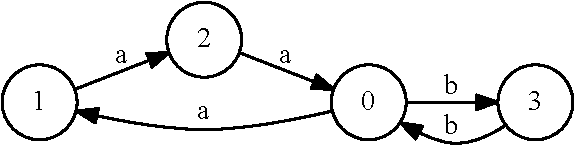
\includegraphics[width=7cm]{pictures/example_graph.pdf}
	\]
	\caption{An example graph.}
	\label{Example_Graph}
\end{figure}

For this graph, we have a same-generation query, formulated as a context-free grammar, which generates a context-free language \mbox{$L=\{a^n b^n~|~n \geq 1\}$}. This grammar is equal to $G = (N, \Sigma, P)$ where:
\begin{itemize}
	\item the set of non-terminals $N = \{S\}$;
	\item the set of terminals $\Sigma = \{a, b\}$;
	\item the set of production rules $P$ is presented on Figure~\ref{ProductionRulesWorsCaseExample}.
\end{itemize}

\begin{figure}[h]
	\[
	\begin{array}{rccl}
	0: & S & \rightarrow & \text{\emph{a}} \ S \ \text{\emph{b}} \\
	1: & S & \rightarrow & \text{\emph{a}} \ \text{\emph{b}} \\ 
	\end{array}
	\]
	\caption{Production rules for the example query grammar.}
	\label{ProductionRulesWorsCaseExample}
\end{figure}

Since our matrix-based algorithms for CFPQ processes only grammars in Chomsky normal form, we first transform the grammar $G$ into an equivalent grammar $G' = (N', \Sigma', P')$ in normal form, where:
\begin{itemize}
	\item the set of non-terminals $N' = \{S, S_1, A, B\}$;
	\item the set of terminals $\Sigma' = \{a, b\}$;
	\item the set of production rules $P'$ is presented on Figure~\ref{ProductionRulesExampleQueryCNF}.
\end{itemize}

\begin{figure}[h]
	\[
	\begin{array}{rccl}
	0: & S & \rightarrow & A \ B \\
	1: & S & \rightarrow & A \ S_1 \\
	2: & S_1 & \rightarrow & S \ B \\
	3: & A & \rightarrow & \text{\emph{a}} \\ 
	4: & B & \rightarrow & \text{\emph{b}} \\ 
	\end{array}
	\]
	\caption{Production rules for the example query grammar in normal form.}
	\label{ProductionRulesExampleQueryCNF}
\end{figure}

The result of context-free path query evaluation w.r.t. the relational query semantics for this example is a set of node pairs \mbox{$(m, n)$}, such that there is a path from the node $m$ to the node $n$, whose labeling forms a word from the language $L$. For example, the node pair \mbox{$(0,0)$} must be in this set, since there is a path from the node $0$ to the node $0$, whose labeling forms a string \mbox{$w = aaaaaabbbbbb = a^6b^6 \in L$}.

The result of context-free path query evaluation w.r.t. the single-path query semantics also contains such a path for each node pair \mbox{$(m, n)$} returned after the context-free path query evaluation w.r.t the relational query semantics. For example, if we want to provide proof of the existence of such a path for the node pair \mbox{$(0,0)$}, the path from the node $0$ to the node $0$, whose labeling forms a string \mbox{$w = a^6b^6$} can be returned. 
\section{Preliminaries} \label{section_preliminaries}
In this section, we introduce the basic notions used throughout the paper.

Let $\Sigma$ be a finite set of edge labels. Define an \textit{edge-labeled directed graph} as a tuple $D = (V, E)$ with $V$ is a set of nodes and $E \subseteq V \times \Sigma \times V$ is a directed edge-relation.  For a path $\pi$ in a graph $D$ we denote $l(\pi)$ --- the unique word obtained by concatenating the labels of the edges along the path $\pi$. Also, we write $n \pi m$ to indicate that a path $\pi$ starts at node $n \in V$ and ends at node $m \in V$.

According to Hellings~\cite{hellingsRelational}, we deviate from the usual definition of a context-free grammar in \textit{Chomsky Normal Form}~\cite{chomsky} by not including a special start non-terminal, which will be specified in the queries to the graph. Since every context-free grammar can be transformed into an equivalent one in Chomsky Normal Form and checking that an empty string is in the language is trivial, then it is sufficient to only consider grammars of the following type. A \textit{context-free grammar} is 3-tuple $G = (N, \Sigma, P)$ where $N$ is a finite set of non-terminals, $\Sigma$ is a finite set of terminals, and $P$ is a finite set of productions of the following forms:

\begin{itemize}
    \item $A \rightarrow B C$, for $A,B,C \in N$,
    \item $A \rightarrow x$, for $A \in N$ and $x \in \Sigma$.   
\end{itemize}

Note that we omit the rules of the form $A \rightarrow \varepsilon$, where $\varepsilon$ denotes an empty string. This does not limit the applicability of further algorithms because checking that an empty string belongs to the context-free language in Chomsky normal form is trivial and only the empty paths $m \pi m$ correspond to an empty string $\varepsilon$.

We use the conventional notation $A \xrightarrow{*} w$ to denote that the string $w \in \Sigma^*$ can be derived from a non-terminal $A$ by some sequence of applying the production rules from $P$. The \textit{language} of a grammar $G = (N,\Sigma,P)$ with respect to a start non-terminal $S \in N$ is defined by $L(G_S) = \{w \in \Sigma^*~|~S \xrightarrow{*} w\}$.

For a given graph $D = (V, E)$ and a context-free grammar $G = (N, \Sigma, P)$, we define \textit{context-free relations} $R_A \subseteq V \times V$, for every $A \in N$, such that $R_A = \{(n,m)~|~\exists n \pi m~(l(\pi) \in L(G_A))\}$.

We define a binary operation on arbitrary subsets $N_1 , N_2$ of $N$ with respect to a context-free grammar $G = (N, \Sigma, P)$ as $N_1 \cdot N_2 = \{A~|~\exists B \in N_1, \exists C \in N_2 \text{ such that }(A \rightarrow B C) \in P\}.$

Using this binary operation as a multiplication on arbitrary subsets of $N$ and union of sets as an addition, we can define a \textit{matrix multiplication}, $a \cdot b = c$, where $a$ and $b$ are matrices of the suitable size that have subsets of $N$ as elements, as $c_{i,j} = \bigcup^{n}_{k=1}{a_{i,k} \cdot b_{k,j}}$.

We define the \textit{transitive closure} of a square matrix $a$ as $a^+ = a^{(1)} \cup a^{(2)} \cup \cdots$ where $a^{(i)} = a^{(i-1)} \cup (a^{(i-1)} \cdot a^{(i-1)})$, $i \ge 2$ and $a^{(1)} = a$.
\section{Matrix-based Algorithm for CFPQ}

Matrix-based algorithm for CFPQ was proposed by Rustam Azimov~\cite{Azimov:2018:CPQ:3210259.3210264}.
This algorithm can be expressed in terms of operations over matrices (see listing~\ref{lst:algo1}), and it is a sufficient advantage for implementation.
It was shown that GPGPU utilization for queries evaluation can significantly improve performance in comparison to other implementations~\cite{Azimov:2018:CPQ:3210259.3210264} even if float matrices are used instead of boolean matrices.

\begin{algorithm}
  \floatname{algorithm}{Listing}
\begin{algorithmic}[1]
\caption{Context-free path quering algorithm}
\label{lst:algo1}
\Function{contextFreePathQuerying}{D, G}

    \State{$n \gets$ the number of nodes in $D$}
    \State{$E \gets$ the directed edge-relation from $D$}
    \State{$P \gets$ the set of production rules in $G$}
    \State{$T \gets$ the matrix $n \times n$ in which each element is $\varnothing$}
    \ForAll{$(i,x,j) \in E$}
    \Comment{Matrix initialization}
        \State{$T_{i,j} \gets T_{i,j} \cup \{A~|~(A \rightarrow x) \in P \}$}
    \EndFor
    \While{matrix $T$ is changing}

        \State{$T \gets T \cup (T \times T)$}
        \Comment{Transitive closure calculation}
    \EndWhile
\State \Return $T$
\EndFunction
\end{algorithmic}
\end{algorithm}

Here $D = (V, E)$ is the input graph and $G = (N,\Sigma,P)$ is the input grammar.
Each cell of the matrix $T$ contains the set of nonterminals such that $N_k \in T[i,j] \iff \exists p = v_i \ldots v_j $---path in $D$, such that $N_k \xRightarrow[G]{*} \omega(p) $, where $\omega(p)$ is a word formed by labels along the path $p$.
Thus, this algorithm solves reachability problem, or, according to Hellings~\cite{hellingsRelational}, process CFPQs by using relational query semantics.

The performance-critical part of this algorithm is matrix multiplication.
Note, that the set of nonterminals is finite, and we can represent the matrix $T$ as a set of boolean matrices: one for each nonterminal.
In this case the matrix update operation is $T_{N_i} \leftarrow T_{N_i} + (T_{N_j} \times T_{N_k})$ for each production $N_i \rightarrow N_j \ N_k$ in $P$.
Thus we can reduce CFPQ to boolean matrices multiplication.
After such transfromation, we can apply the next optimization: we can skip update if the matrices $T_{N_j}$ and $T_{N_k}$ have not been changed at the previous iteration.

Thus, the most important part is the efficient implementation of operations over boolean matrices, and in this work we compare effects of utilization of different approaches to matrices multiplication.
All our implementations are based on the optimized version of the algorithm.

\section{Matrix-based CFPQ for Single-Path Semantics}
In this section, we propose the matrix-based algorithm for CFPQ w.r.t. the single-path query semantics (see listing~\ref{lst:algo2}). This algorithm constructs the set of matrices $T$ with PathIndexes as elements.
{\small
	\begin{algorithm}
		\floatname{algorithm}{Listing}
		\begin{algorithmic}[1]
			\caption{CFPQ algorithm w.r.t. single-path query semantics}
			\label{lst:algo2}
			\Function{evalCFPQ}{$D=(V,E), G=(N,\Sigma,P)$}
			\State{$n \gets$ |V|}
			\State{$T \gets \{T^{A_i} \mid A_i \in N, T^{A_i}$ is a matrix $n \times n$, $T^{A_i}_{k,l} \gets \bot$ \} }
			\ForAll{$(i,x,j) \in E$, $A_k \mid A_k \to x \in P$}
			%\Comment{Matrices initialization}
			%\For{$A_k \mid A_k \to x \in P$}
			{$T^{A_k}_{i,j} \gets (i,j,i,1,1)$}
			%\EndFor
			\EndFor
			\For{$A_k \mid A_k \to \varepsilon \in P$}
			{$T^{A_k}_{i,i} \gets (i,i,i,1,0)$}
			\EndFor
			
			\While{any matrix in $T$ is changing}
			%\Comment{Transitive closure calculation}
			\For{$A_i \to A_j A_k \in P$}
			{ $T^{A_i} \gets T^{A_i} + (T^{A_j} \odot T^{A_k})$ } 
			\EndFor
			\EndWhile
			\State \Return $T$
			\EndFunction
		\end{algorithmic}
	\end{algorithm}
}

After constructing the set of matrices $T$ for every node pair $i, j$ and nonterminal $A$ we can extract a path $i \pi j$ from $i$ to $j$ such that $A \xRightarrow[G]{*} l(\pi)$ if such path exists. We also propose the algorithm (see listing~\ref{lst:algo3}) for extracting one of those paths which forms a string with minimal height of derivation tree. Our algorithm returns the empty path $[]$ only if $i = j$ and $A \to \varepsilon \in P$. Note that if the PathIndex for given $i,j,A$ is equal to $\bot$ then our algorithm returns a special path $\pi_{\emptyset}$ to denote that such a path does not exist.

{\small
	\begin{algorithm}
		\floatname{algorithm}{Listing}
		\begin{algorithmic}[1]
			\caption{Path extraction algorithm}
			\label{lst:algo3}
			\Function{extractPath}{$i, j, A, T=\{T^{A_i}\}, G=(N,\Sigma,P)$}
			\State{$index \gets T^{A}_{i,j}$ }
			
			\If{$index = \bot$}
			\State \Return $\pi_{\emptyset}$
			\Comment{Such a path does not exist}
			\EndIf
			
			\If{$index.height = 1$}
			\If{$index.length = 0$}
			\State \Return $[]$
			\Comment{Return an empty path}
			\EndIf
			\ForAll{$ x \mid (i,x,j) \in E$}
			\If{$A \to x \in P$}
			\State \Return $[(i,x,j)]$
			\Comment{Return a path of length one}
			\EndIf
			\EndFor
			\EndIf
			
			\ForAll{$A \to B C \in P$}
			\State{$index_B \gets T^{B}_{i,index.middle}$ }
			\State{$index_C \gets T^{C}_{index.middle,j}$ }			
			\If{$(index_B \neq \bot) \wedge (index_C \neq \bot)$}
			\State{$maxH \gets max(index_B.height, index_C.height)$ }
			\If{$index.height = maxH + 1$}
			
						
			\State{$\pi_1 \gets$ \Call{extractPath}{$i, index.middle, B, T, G$}}
			\State{$\pi_2 \gets$ \Call{extractPath}{$index.middle, j, C, T, G$}}
			\State \Return $\pi_1 + \pi_2$
			\EndIf
			\EndIf
			\EndFor
			\EndFunction
		\end{algorithmic}
	\end{algorithm}
}

\subsection{Correctness}

Let $T^{(p)} = \{T^{(p), A_i}\}$ be a constructed matrix $T$ by the algorithm in listing~\ref{lst:algo2} after $p-1$ loop iterations for $p \geq 2$, and $T^{(1)} = \{T^{(1), A_i}\}$ be a constructed matrix $T$ by this algorithm after initialization in lines 3-5. Note that the matrix $T$ returned by this algorithm is equal to $\sum_{p = 1}^{\infty} T^{(p)}$. Then the following lemma and theorem hold.

\begin{lemma}\label{lemma:correctness}
	Let $D = (V,E)$ be a graph, let $G =(N,\Sigma,P)$ be a grammar. Then for any $i, j$ and for any non-terminal $A \in N$, $index = T^{(p),A}_{i,j}$ and $index = (i,j,k,h,l) \neq \bot$ iff $(i,j) \in R_A$ and $i \pi j$, such that there is a derivation tree of the minimal height $h \leq p$ for the string $l(\pi)$  of length $l$ and a context-free grammar $G_A = (N,\Sigma,P,A)$.
\end{lemma}
\begin{proof}(Proof by Induction)
	
	\textbf{Base case}: Show that the lemma holds for $p = 1$. For any $i, j$ and for any non-terminal $A \in N$, $(i,j,k,h,l) = T^{(1), A}_{i,j}$ iff there is either $i \pi j$ of length $1$ that consists of a unique edge $e$ from the node $i$ to the node $j$ and $(A \rightarrow x) \in P$, where $x = l(\pi)$, or $i = j$ and $(A \rightarrow \varepsilon) \in P$, where $\varepsilon = l(\pi)$. Therefore $(i,j) \in R_A$ and there is a derivation tree of the minimal height $h = p = 1$, shown on Figure~\ref{tree1}, for the string $x$ and a context-free grammar $G_A = (N,\Sigma,P,A)$. Thus, it has been shown that the lemma holds for $p = 1$.
	
	\begin{figure}[h!]
		\centering
		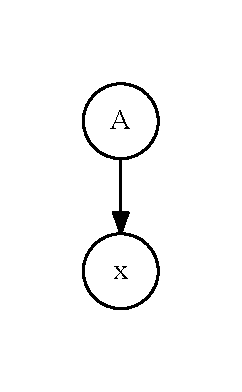
\includegraphics[width=2cm]{pictures/tree1.pdf}
		\caption{The derivation tree of the minimal height $p = 1$ for the string $x = l(\pi)$ where $x \in \Sigma \cup \{\varepsilon\}$.}
		\label{tree1}
	\end{figure}
	
	\textbf{Inductive step}: Assume that the lemma holds for any $p \leq (q - 1)$ and show that it also holds for $p = q$, where $q \geq 2$.
	
	The index $(i,j,k,h,l) = T^{(q),A}_{i,j}$ iff there is exists a rule $(A \to B C) \in P$ such that $(i,j,k,h,l) = M_{i,j}$ where $$M = T^{(q-1),A} + (T^{(q-1),B} \odot T^{(q-1),C}).$$ 
	
	Let $(i,j,k,h,l) = T^{(q-1),A}_{i,j}$. By the inductive hypothesis, $(i,j,k,h,l) = T^{(q-1),A}_{i,j}$ iff $(i,j) \in R_A$ and there exists $i \pi j$, such that there is a derivation tree of the minimal height $h \leq (q-1)$ for the string $l(\pi)$ and a context-free grammar $G_A = (N,\Sigma,P,A)$. The statement of the lemma holds for $p = q$ since the height $h$ of this tree is also less than or equal to $q$.
	
	Now, let $(i,j,k,h,l) = (T^{(q-1),B} \odot T^{(q-1),C})_{i,j}$. By the definition of the binary operation $\odot$, $(i,j,k,h,l) = (T^{(q-1),B} \odot T^{(q-1),C})_{i,j}$ iff there are $r=k$, $(i,r,\_,h_1,l_1) = T^{(q-1),B}_{i,r}$ and $(r,j,\_,h_2,l_2) = T^{(q-1),C}_{r,j}$, such that $q = max(h_1, h_2) + 1$, $l = l_1 + l_2$. Hence, by the inductive hypothesis, there are $i \pi_1 r$ and $r \pi_2 j$, such that $(i,r) \in R_B$ and $(r,j) \in R_C$, and there are the derivation trees $T_B$ and $T_C$ of minimal heights $h_1 \leq (q-1)$ and $h_2 \leq (p-1)$ for the strings $w_1 = l(\pi_1)$, $w_2 = l(\pi_2)$ and the context-free grammars $G_B$, $G_C$ respectively. Thus, the concatenation of paths $\pi_1$ and $\pi_2$ is $i \pi j$, where $(i,j) \in R_A$ and there is a derivation tree of the minimal height $h = 1 + max(h_1, h_2)$, shown on Figure~\ref{tree2}, for the string $w = l(\pi)$ of length $l = l_1 + l_2$ and a grammar $G_A$.
	\begin{figure}[h!]
		\centering
		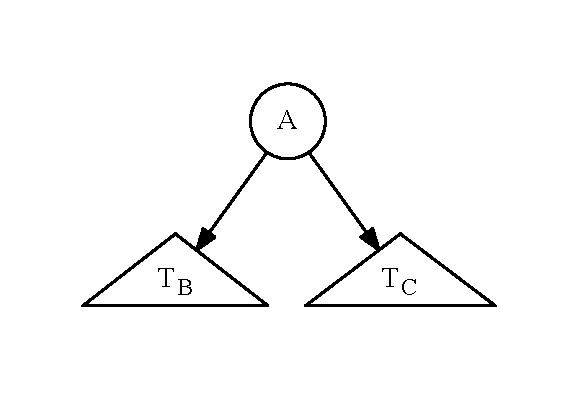
\includegraphics[width=5cm]{pictures/tree2.pdf}
		\caption{The derivation tree of the minimal height $h = 1 + max(h_1, h_2)$ for the string $w = l(\pi)$, where $T_B$ and $T_C$ are the derivation trees for strings $w_1$ and $w_2$ respectively.}
		\label{tree2}
	\end{figure}
	
	The statement of the lemma holds for $p = q$ since the minimal height $h = 1 + max(h_1, h_2) \leq q$. This completes the proof of the lemma.
\end{proof}

\begin{mytheorem}\label{thm:correct}
	Let $D = (V,E)$ be a graph and let $G =(N,\Sigma,P)$ be a grammar. Then for any $i, j$ and for any non-terminal $A \in N$, $index = T^A_{i,j}$ and $index = (i,j,k,h,l) \neq \bot$ iff $(i,j) \in R_A$ and $i \pi j$, such that there is a derivation tree of the minimal height $h$ for the string $l(\pi)$ of length $l$ and a context-free grammar $G_A = (N,\Sigma,P,A)$.
\end{mytheorem}
\begin{proof}
	
	Since the matrix $T = \sum_{p = 1}^{\infty} T^{(p)}$ for any $i, j$ and for any non-terminal $A \in N$, $index = T^A_{i,j}$ and $index = (i,j,k,h,l) \neq \bot$ iff there is $p \geq 1$, such that $index \in T^{(p),A}_{i,j}$. By the lemma~\ref{lemma:correctness}, $index = T^{(p),A}_{i,j}$ iff $(i,j) \in R_A$ and $i \pi j$, such that there is a derivation tree of the minimal height $h \leq p$ for the string $l(\pi)$  of length $l$ and a context-free grammar $G_A = (N,\Sigma,P,A)$. This completes the proof of the theorem.
\end{proof}

Now, using the theorem~\ref{thm:correct} and induction on the length of the path, it can be easily shown that the following theorem holds.

\begin{mytheorem}\label{thm:correct_extraction}
	Let $D = (V,E)$ be a graph, let $G =(N,\Sigma,P)$ be a grammar and $T$ be a set of matrices returned by the algorithm in listing~\ref{lst:algo2}. Then for any $i, j$ and for any non-terminal $A \in N$ such that $index = T^A_{i,j}$ and $index = (i,j,k,h,l) \neq \bot$, the algorithm in listing~\ref{lst:algo3} for these parameters will return a path $i \pi j$ such that $(i,j) \in R_A$ and there is a derivation tree of the minimal height $h$ for the string $l(\pi)$ of length $l$ and a context-free grammar $G_A = (N,\Sigma,P,A)$.
\end{mytheorem}

We can, therefore, determine whether $(i,j) \in R_A$ by asking whether $T^A_{i,j} = \bot$. Also, we can extract such a path which forms a string with a derivation tree of minimal height by using our algorithm in listing~\ref{lst:algo3}. Thus, we show how the context-free path query evaluation w.r.t. the single-path semantics can be solved in terms of matrix operations.

\subsection{Complexity}

Denote the number of elementary operations executed by the algorithm of multiplying two $n \times n$ matrices with PathIndexes as $MM(n)$. Also, denote the number of elementary operations, executed by the matrix element-wise + operation of two $n \times n$ matrices with PathIndexes as $MA(n)$. Since the line \textbf{7} of the algorithm in listing~\ref{lst:algo2} is executed no more than $|V|^2|N|$ times, the following theorem holds.

\begin{mytheorem}\label{thm:time}
	Let $D = (V,E)$ be a graph and let $G =(N,\Sigma,P)$ be a grammar. The algorithm in listing~\ref{lst:algo2} calculates the set of matrices $T$ in $O(|V|^2|N|^3(MM(|V|) + MA(|V|)))$.
\end{mytheorem}

Also, denote the time complexity of the access to the PathIndex in the $n \times n$ matrix as $Access(n)$. Then the following theorem on the time complexity of the path extraction algorithm holds.

\begin{mytheorem}\label{thm:time_extraction}
	Let $D = (V,E)$ be a graph, let $G =(N,\Sigma,P)$ be a grammar and $T$ be a set of matrices returned by the algorithm in listing~\ref{lst:algo2}. Then for any $i, j$ and for any non-terminal $A \in N$ such that $index = T^A_{i,j}$ and $index = (i,j,k,h,l) \neq \bot$, the algorithm in listing~\ref{lst:algo3} for these parameters calculates a path $i \pi j$ in $O(l \times N \times Access(|V|))$.
\end{mytheorem}

\subsection{An Example}
In this section, we provide a step-by-step demonstration of the proposed algorithms. For this, we consider the example with the worst-case time complexity.

The \textbf{example query} is based on the context-free grammar $G = (N, \Sigma, P)$ of the worst-case example query where:
\begin{itemize}
	\item the set of non-terminals $N = \{S\}$;
	\item the set of terminals $\Sigma = \{a, b\}$;
	\item the set of production rules $P$ is presented on Figure~\ref{ProductionRulesWorsCaseExample}.
\end{itemize}

\begin{figure}[h]
	\[
	\begin{array}{rccl}
	0: & S & \rightarrow & \text{\emph{a}} \ S \ \text{\emph{b}} \\
	1: & S & \rightarrow & \text{\emph{a}} \ \text{\emph{b}} \\ 
	\end{array}
	\]
	\caption{Production rules for the worst-case example.}
	\label{ProductionRulesWorsCaseExample}
\end{figure}

Since the proposed algorithm processes only grammars in Chomsky normal form, we first transform the grammar $G$ into an equivalent grammar $G' = (N', \Sigma', P')$ in normal form, where:
\begin{itemize}
	\item the set of non-terminals $N' = \{S, S_1, A, B\}$;
	\item the set of terminals $\Sigma' = \{a, b\}$;
	\item the set of production rules $P'$ is presented on Figure~\ref{ProductionRulesExampleQueryCNF}.
\end{itemize}

\begin{figure}[h]
	\[
	\begin{array}{rccl}
	0: & S & \rightarrow & A \ B \\
	1: & S & \rightarrow & A \ S_1 \\
	2: & S_1 & \rightarrow & S \ B \\
	3: & A & \rightarrow & \text{\emph{a}} \\ 
	4: & B & \rightarrow & \text{\emph{b}} \\ 
	\end{array}
	\]
	\caption{Production rules for the example query grammar in normal form.}
	\label{ProductionRulesExampleQueryCNF}
\end{figure}

We run the query on a graph, presented in Figure~\ref{Example_Graph}. We provide a step-by-step demonstration of the work with the given graph $D$ and grammar $G'$ of the algorithm in listing~\ref{lst:algo2}. After the matrix initialization in lines \textbf{3-5} of this algorithm, we have a matrix $T^{(1)}$, presented on Figure~\ref{ExampleQueryInitMatrix}.

\begin{figure}[h]
	\[
	T^{(1),A} = \begin{pmatrix}
	\bot & (0,1,0,1,1)       & \bot & \bot       \\
	\bot & \bot & (1,2,1,1,1)       & \bot \\
	(2,0,2,1,1)       & \bot & \bot & \bot \\
	\bot       & \bot & \bot & \bot \\
	\end{pmatrix}
	\]
	\[
	T^{(1),B} = \begin{pmatrix}
	\bot & \{A\}       & \bot & (0,3,0,1,1)       \\
	\bot & \bot & \{A\}       & \bot \\
	\{A\}       & \bot & \bot & \bot \\
	(3,0,3,1,1)      & \bot & \bot & \bot \\
	\end{pmatrix}
	\]
	\caption{The initial matrix for the example query. The PathIndexes $T^{(1),S_1}_{i,j}$ and $T^{(1),S}_{i,j}$ are equal to $\bot$ for every $i,j$.}
	\label{ExampleQueryInitMatrix}
\end{figure}

After the initialization, the only matrices which will be updated are $T^{S_1}$ and $T^{S}$. These matrices obtained after the first loop iteration is shown in Figure~\ref{ExampleQueryFirstIteration}.

\begin{figure}[h]
	\[
	T^{(2),S} = \begin{pmatrix}
	\bot & \bot       & \bot & \bot       \\
	\bot & \bot & \bot       & \bot \\
	\bot       & \bot & \bot & (2,3,0,2,2) \\
	\bot       & \bot & \bot & \bot \\
	\end{pmatrix}
	\]
	\caption{The first iteration of computing the transitive closure for the example query. The PathIndexes $T^{(1),S_1}_{i,j}$ are equal to $\bot$ for every $i,j$.}
	\label{ExampleQueryFirstIteration}
\end{figure}

When the algorithm at some iteration finds new paths for some nonterminal in the graph $D$, then it adds corresponding PathIndexes to the matrix for this nonterminal. For example, after the first loop iteration, PathIndex $(2,3,0,2,2)$ is added to the matrix $T^{S}$. This PathIndex is added to the element with a row index $i = 2$ and a column index $j = 3$. This means, that there is $i\pi j$ (a path $\pi$ from the node 2 to the node 3), such that $S \xRightarrow[G]{*} l(\pi)$, this path obtained by concatenation of smaller paths via node 0, the length of the path is equal to 2, and the derivation tree for the string $l(pi)$ has a height 2.

The calculation of the transitive closure is completed after $k$ iterations, when a fixpoint is reached: $T^{(k)} = T^{(k+1)}$. For the example query, $k = 13$ since $T_{13} = T_{14}$. The resulted matrices are presented on Figure~\ref{ExampleQueryFinalMatrices}.

\begin{figure}[h]
	\[
	T^{(14),S} = \begin{pmatrix}
	(0,0,1,12,12) & \bot       & \bot & (0,3,1,6,6)       \\
	(1,0,2,4,4) & \bot & \bot       & (1,3,2,10,10) \\
	(2,0,0,8,8)       & \bot & \bot & (2,3,0,2,2) \\
	\bot       & \bot & \bot & \bot \\
	\end{pmatrix}
	\]
	
	\[
	T^{(14),S_1} = \begin{pmatrix}
	(0,0,3,7,7)  & \bot       & \bot & (0,3,0,13,13)       \\
	(1,0,3,11,11) & \bot & \bot       & (1,3,0,5,5) \\
	(2,0,3,3,3)       & \bot & \bot & (2,3,0,9,9) \\
	\bot       & \bot & \bot & \bot \\
	\end{pmatrix}
	\]
	\caption{The final matrices after computing the transitive closure for the example query.}
	\label{ExampleQueryFinalMatrices}
\end{figure}

Thus, the result of the algorithm in listing~\ref{lst:algo2} for the example query are the matrices on Figures~\ref{ExampleQueryInitMatrix} and \ref{ExampleQueryFinalMatrices}. Now, after constructing the transitive closure, we can construct the context-free relations $R_A$. These relations for each non-terminal of the grammar $G'$ are presented on Figure~\ref{ExampleQueryCFRelations}.

\begin{figure}[h]
	\begin{eqnarray*}
		R_S&=&\{(0,0),(0,3),(1,0),(1,3),(2,0),(2,3)\},\\
		R_{S_1}&=&\{(0,0),(0,3),(1,0),(1,3),(2,0),(2,3)\},\\
		R_{A}&=&\{(0,1),(1,2),(2,0)\}, \\
		R_{B}&=&\{(0,3), (3,0)\}.
	\end{eqnarray*}
	\caption{Context-free relations for the example query.}
	\label{ExampleQueryCFRelations}
\end{figure}

In the context-free relation $R_S$, we have all node pairs corresponding to paths, whose labeling is in the language $L(G_S) = \{a^n b^n| n \geq 1\}$. Using the algortihm in listing~\ref{lst:algo3} we can restore paths for each node pair from context-free relations. For example, given $i=j=0$, nonterminal $S$, set of resulted matrices $T$, and context-free grammar $G'$, the algorithm in listing~\ref{lst:algo3} returns a path $0\pi 0$ whose labeling forms a string $l(\pi) = a^6 b^6$. The length of path $\pi$ is equal to 12 and the height of the derivation tree for $l(\pi)$ is equal to 12, which is consistent with the corresponding PathIndex $T^{(14),S}_{0,0}$.
\section{Implementation}

We implement the matrix-based algorithm for CFPQ by using several different programming languages and tools.
We aim to investigate the effects of the following features of an implementation.
\begin{itemize}
\item \textbf{GPGPU utilization.}
It is well-known that GPGPUs are suitable for matrices operations, but the performance of the whole solution depends on the implementation details. For example, overhead on data transferring may negate the effect of parallel computations.
Can GPGPUs utilization for CFPQ improve performance in comparison with the CPU version?

\item \textbf{Existing libraries utilization} is a good practice in software engineering.
Is it possible to achieve higher performance by means of existing libraries for matrices operations or do we need to create our own solution to get more control?

\item \textbf{Low-level programming}.
GPGPU programming traditionally involves low-level programming in C-based languages (CUDA C, OpenCL C).
But can we achieve a high-performance solution with high-level languages such as Python?

\item \textbf{Sparce matrices.} Real graphs are often sparse.
Can we gain more performance improvement by using sparse matrix representation for CFPQ?

\end{itemize}

We provide the following implementations for investigation.

\begin{itemize}
  \item CPU-based solutions
%  \begin{itemize}

    \textbf{[Scipy]} Sparse matrices multiplication by using Scipy~\cite{scipy} in Python programming language.

    \textbf{[M4RI]} Dense matrices multiplication by using m4ri\footnote{Actually we use pull request which is not merged yet: \url{https://bitbucket.org/malb/m4ri/pull-requests/9/extended-m4ri-to-multiplication-over-the/diff}. The original library implements operations over $GF(2)$, and this pull request contains operations over boolean semiring}~\cite{M4RI} library which implements the Method of Four Russians~\cite{arlazarov1970economical} in C language.
    This library is choosen because it is a performant implementation of the Method of Four Russians~\cite{albrechtefficient}.
  %\end{itemize}
  \item GPGPU-based solutions

    \textbf{[GPU4R]} Our own implementation of the Method of Four Russians in CUDA C.

    \textbf{[GPU\_N]} Our own implementation of the na\"ive boolean matrix multiplication in CUDA C with boolean values treated as bits and packed into \texttt{uint\_32}.

    \textbf{[GPU\_Py]} Manual implementation of na\"ive boolean matrix multiplication in Python by using numba compiler\footnote{Numba is a JIT compiler which supports GPGPU for a subset of Python programming. Official page: \url{http://numba.pydata.org/}. Access date: 03.05.2019}.
    Boolean values are packed into \texttt{uint\_32}.

\end{itemize}

As far as a set of matrices and its size can be calculated at the start of computations, all the GPGPU based implementations allocate all required memory on the GPGPU once, at the start of computations.
This significantly reduces the overhead on data transferring: all input data is loaded to the GPGPU at the start, and the result is loaded from the GPGPU to the host at the end.
As a result, there is no active data transferring and memory allocating during query computation.

\section{Dataset description}

We created and published a dataset for CFPQ algorithms evaluation.
This dataset contains both the real-world data and synthetic data for different specific cases, such as the theoretical worst case, or the worst cases specific to matrices representations.

Our goal is to evaluate querying algorithms, not graph storages or graph databases, so all data is presented in a text-based format to simplify usage in different environments.
Grammars are in Chomsky Normal Form, and graphs are represented as a list of triples (edges).
Some details of the data representation can be found in the Appendix.

The variants of the \textit{same generation query}~\cite{FndDB} are an important example of queries that are context-free but not regular, so we use this type of queries in our evaluation.
The dataset includes data for the following cases.
Each case is a pair of a set of graphs and a set of grammars: each query (grammar) should be applied to each graph.

\textbf{[RDF]} The set of the real-world RDF files (ontologies) from~\cite{RDF} and two variants of the same generation query which describes hierarchy analysis.
The first query is the grammar $G_4$:
\[
 \begin{array}{lcl}
   s  \rightarrow \textit{SCOR} \ s \ \textit{SCO}   & \quad & s  \rightarrow \textit{TR} \ s \ \textit{T}     \\
   s  \rightarrow \textit{SCOR} \ \textit{SCO}       & \quad & s  \rightarrow  \textit{TR}  \ \textit{T}

 \end{array}
 \]
The second one is the grammar $G_5$: $s \rightarrow \textit{SCOR} \ s \ \textit{SCO} \ | \  \textit{SCO}$.

\textbf{[Worst]} The theoretical worst case for CFPQ time complexity proposed by Hellings~\cite{hellingsPathQuerying}: the graph is two cycles of coprime lengths with a single common vertex.
The first cycle is labeled by the open bracket and the second cycle is labeled by the close bracket.
Query is a grammar for the $A^nB^n$ language.
The example of such graph and grammar is presented in figure~\ref{fig:grammar_example}.

\begin{figure}[h]
    \centering
    \begin{subfigure}[b]{0.20\textwidth}
        \centering
        \[
         \begin{array}{l}
           s \rightarrow A \ s \ B \\
           s \rightarrow A \ B
         \end{array}
         \]
        \caption{Grammar $G_1$ for $\{A^n B^n\}$}
    \end{subfigure}%
    ~\quad
    \begin{subfigure}[b]{0.24\textwidth}
        \centering
        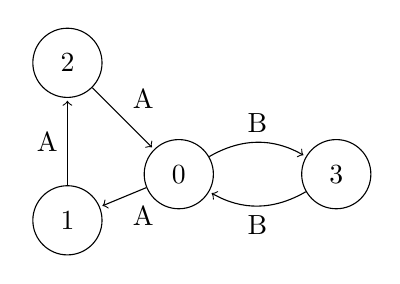
\begin{tikzpicture}[shorten >=1pt,node distance=2cm,on grid,auto]
   \node[state] (q_1)   {$1$};
   \node[state] (q_2) [above=of q_1] {$2$};
   \node[state] (q_3) [above right=of q_1, below right=of q_2] {$0$};
   \node[state] (q_4) [right=of q_3] {$3$};
    \path[->]
    (q_1) edge  node {A} (q_2)
    (q_2) edge  node {A} (q_3)
    (q_3) edge  node {A} (q_1)
    (q_3) edge[bend left, above]  node {B} (q_4)
    (q_4) edge[bend left, below]  node {B} (q_3);
\end{tikzpicture}

        \caption{Input graph $D_1$ for the worst case with \texttt{A} as the open bracket, and \texttt{B} as the close bracket}
        \label{fig:worstCaseGraph}
    \end{subfigure}%
    \caption{Graph and grammar for the worst case}
    \label{fig:grammar_example}
\end{figure}


\textbf{[Full]} The case when the input graph is sparse, but the result is a full graph.
Such a case may be hard for sparse matrices representations.
As an input graph, we use a cycle, all edges of which are labeled by the same token.
As a query we use two grammars which describe the sequence of tokens of arbitrary length: the simple ambiguous grammar $G_2$: $s \rightarrow  s \ s \ | \ A$,  and the highly ambiguous grammar $G_3$: $s \rightarrow s \ s \ s \ | \ A$.

\textbf{[Sparse]} Sparse graphs from~\cite{fan2018scaling} are generated by the GTgraph graph generator, and emulate realistic sparse data.
Names of these graphs have the form \texttt{Gn-p}, where \texttt{n} corresponds to the total number of vertices, and \texttt{p} is the probability that some pair of vertices is connected.
The query is the same generation query represented by the grammar $G_1$ (figure~\ref{fig:grammar_example}).

\section{Evaluation}

We evaluate the implemented algorithm on both regular and context-free path queries in order to demonstrate applicability of the proposed solution.
Namely, goals of the evaluation are following.
\begin{enumerate}
	\item Investigate the practical applicability of RPQ evaluation by the proposed algorithm.
	\item Compare Azimov's algorithm for reachability CFPQ and the proposed algorithm.
	\item Investigate the practical applicability of paths extraction algorithm for both regular and context-free queries.
\end{enumerate}

For evaluation, we use a PC with Ubuntu 18.04 installed.
It has Intel core i7-6700 CPU, 3.4GHz, and DDR4 64Gb RAM.
As far as we evaluate only algorithm execution time, we store each graph fully in RAM as its adjacency matrix in sparse format.
Note, that graph loading time is not included in the result time of evaluation.	

\subsection{RPQ Evaluation}

In oder to investigate applicability of the proposed algorithm for RPQ over real-world graphs we collect a set of real-world and synthetic graphs and evaluate queries generated by using the most popular templates for RPQs.

\subsubsection{Dataset}

Brief description of collected graphs are presented in Table~\ref{tbl:graphs_for_rpq}.
Namely, the dataset consists of several parts.
The first one is a set of LUBM graphs\footnote{Lehigh University Benchmark (LUBM) web page: \url{http://swat.cse.lehigh.edu/projects/lubm/}. Access date: 07.07.2020.}~\cite{10.1016/j.websem.2005.06.005} with a different number of vertices.
The second one is a graphs from Uniprot database\footnote{Universal Protein Resource (UniProt) web page: \url{https://www.uniprot.org/}. All files used for evaluation can be downloaded here: \url{ftp://ftp.uniprot.org/pub/databases/uniprot/current_release/rdf/}. Access date: 07.07.2020.}: \textit{proteomes}, \textit{taxonomy} and \textit{uniprotkb}.
The last part is a RDF files \textit{mappingbased\_properties} from DBpedia\footnote{DBpedia project web site: \url{https://wiki.dbpedia.org/}. Access date: 07.07.2020.} and \textit{geospecies}\footnote{The Geospecies RDF: \url{https://old.datahub.io/dataset/geospecies}. Access date: 07.07.2020.}.
These graphs represent data from different areas and they are frequently used for graph querying algorithms evaluation.

\begin{table}
{
\rowcolors{2}{black!2}{black!10}
\begin{tabular}{|l|c|c|}
\hline
Graph & \#V & \#E \\
\hline
\hline 
LUBM1k  & 120 926 & 484 646 \\
LUBM3.5k  & 358 434 & 144 9711 \\
LUBM5.9k  & 596 760 & 2 416 513 \\
LUBM1M   & 1 188 340 & 4 820 728 \\
LUBM1.7M & 1 780 956 & 7 228 358 \\
LUBM2.3M & 2 308 385 & 9 369 511 \\
\hline
Uniprotkb & 6 442 630 & 24 465 430 \\
Proteomes & 4 834 262 & 12 366 973 \\
Taxonomy & 5 728 398 & 14 922 125 \\
\hline
Geospecies & 450 609 & 2 201 532 \\
Mappingbased\_properties & 8 332 233 & 25 346 359 \\
\hline
\end{tabular}
}
\caption{Graphs for RPQ evaluation}
\label{tbl:graphs_for_rpq}
\end{table}


Queries for evaluation was generated by using templates of the most popular RPQs which are collected from~
\cite{Pacaci2020RegularPQ} (Table 2) and~\cite{Wang2019} (some of complex queries from Table 5), and are presented in table~\ref{tbl:queries_templates}.
We generate 10 queries for each template and each graph using the most frequent relations from the given graph randomly\footnote{Used generator is available as part of CFPQ\_data project: \url{https://github.com/JetBrains-Research/CFPQ_Data/blob/master/tools/gen_RPQ/gen.py}. Access data: 07.07.2020.}. 
For all LUBM graphs common set of queries was generated in order to investigate scalability of the proposed algorithm.

\begin{table}
{\small
\renewcommand{\arraystretch}{1.25}
\rowcolors{2}{black!2}{black!10}
\begin{tabular}{|c|c||c|c|}
\hline

Name & Query & Name & Query \\
\hline
\hline 
$Q_1$   & $a^*$                               & $Q_9^5$    & $(a \mid b \mid c \mid d \mid e)^+$                     \\
$Q_2$   & $a\cdot b^*$                        & $Q_{10}^2$ & $(a \mid b) \cdot c^*$                                  \\
$Q_3$   & $a \cdot b^* \cdot c^*$             & $Q_{10}^3$ & $(a \mid b \mid c)  \cdot d^*$                          \\
$Q_4^2$ & $(a \mid b)^*$                      & $Q_{10}^4$ & $(a \mid b \mid c \mid d)  \cdot e^*$                   \\
$Q_4^3$ & $(a \mid b \mid c)^*$               & $Q_{10}^5$ & $(a \mid b \mid c \mid d \mid e)  \cdot f^*$            \\
$Q_4^4$ & $(a \mid b \mid c \mid d)^*$        & $Q_{10}^2$ & $a \cdot b$                                             \\
$Q_4^5$ & $(a \mid b \mid c \mid d \mid e)^*$ & $Q_{11}^3$ & $a \cdot b \cdot c$                                     \\
$Q_5$   & $a \cdot b^* \cdot c$               & $Q_{11}^4$ & $a \cdot b \cdot c \cdot d$                             \\
$Q_6$   & $a^* \cdot b^*$                     & $Q_{11}^5$ & $a \cdot b \cdot c \cdot d \cdot f$                     \\
$Q_7$   & $a \cdot b \cdot c^*$               & $Q_{12}$   & $(a \cdot b)^+ \mid  (c \cdot d)^+$                     \\
$Q_8$   & $a? \cdot b^*$                      & $Q_{13}$   & $(a \cdot(b \cdot c)^*)^+ \mid  (d \cdot f)^+$          \\
$Q_9^2$ & $(a \mid b)^+$                      & $Q_{14}$   & $(a \cdot b \cdot (c \cdot d)^*)^+  \cdot (e \mid f)^*$ \\
$Q_9^3$ & $(a \mid b \mid c)^+$               & $Q_{15}$   & $(a \mid b)^+ \cdot (c \mid d)^+$                       \\
$Q_9^4$ & $(a \mid b \mid c \mid d)^+$        & $Q_{16}$   & $a \cdot b \cdot (c \mid d \mid e)$                     \\
\hline
\end{tabular}
}
\caption{Queries' templates for RPQ evaluation}
\label{tbl:queries_templates}
\end{table}


\subsubsection{Results}

For reachability index creation average time of 5 runs is presented.

Reachability index creation time for each query for LUBM graphs set is presented in figure~\ref{fig:lubm_all_qs}.
We can observe linear !!!! dependency of evaluation time on graph size.
Also we can see, that query evaluation time depends on query: there are queries which evaluate less then 1 second even for biggest graph ($Q_2$, $Q_5$, $Q_{11}^2$, $Q_{11}^3$), while worst time is 6.26 seconds ($Q_{14}$).
Anyway, we can argue that in this case our algorithm demonstrates reasonable time to be applied for real-world data analysis, because it is comparable with recent results on the same problem for LUBM querying by using distributed system over 10 nodes~\cite{Wang2019}, while we use only one node. 
Note, that accurate comparison of different approaches is a huge interesting work for the future.

\begin{figure}
   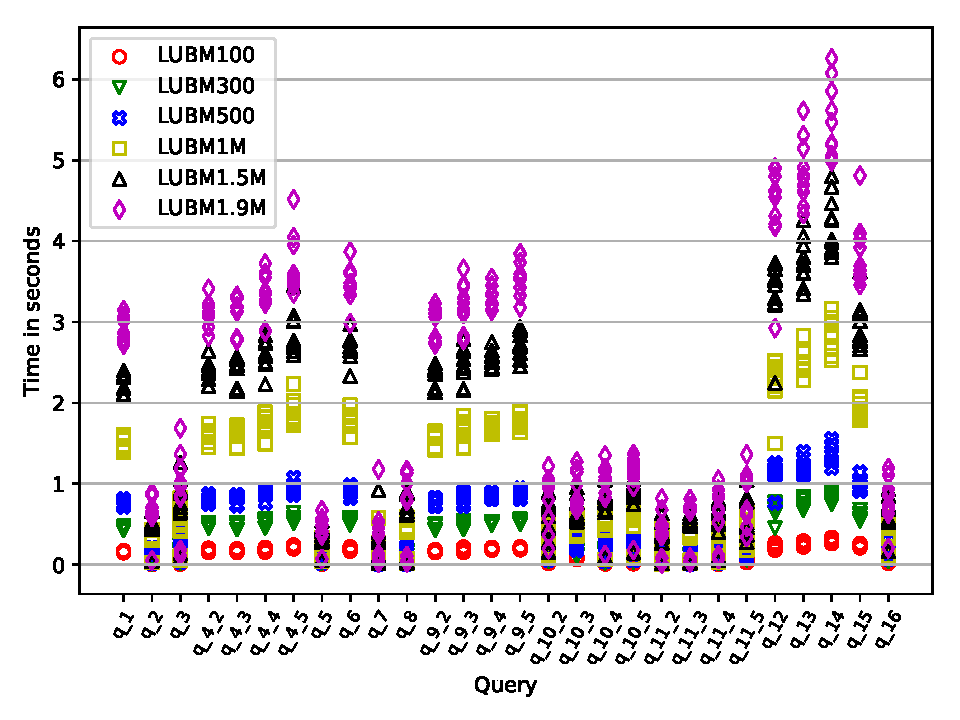
\includegraphics[width=0.48\textwidth]{data/LUBM_all.pdf}
   \caption{Reachability index creation time for LUBM graphs}
   \label{fig:lubm_all_qs}
\end{figure}

Reachability index creation time for each query for for real-world graphs is presented in figure~\ref{fig:other_all_qs}.
We can see that query evaluation time depends on graph inner structure. 
First of all, in some cases handling of small graph requires more time, then handling bigger graph.
For example, $Q_{10}^4$: querying the \textit{geospecies} graph (450k vertices) in some cases requires more time than querying of \textit{mappingbased\_properties} (8.3M vertices) and \textit{taxonomy} (5.7M vertices).
On the other hand, \textit{taxonomy} querying in relatively big number of cases requires significantly more time, than querying of other graphs, while \textit{taxonomy} is not a biggest graph. 
Finally, we can see, that in big number of cases query execution time requires less then 10 seconds, even for big graph, and no queries which require more then 52.17 seconds. 

\begin{figure}
   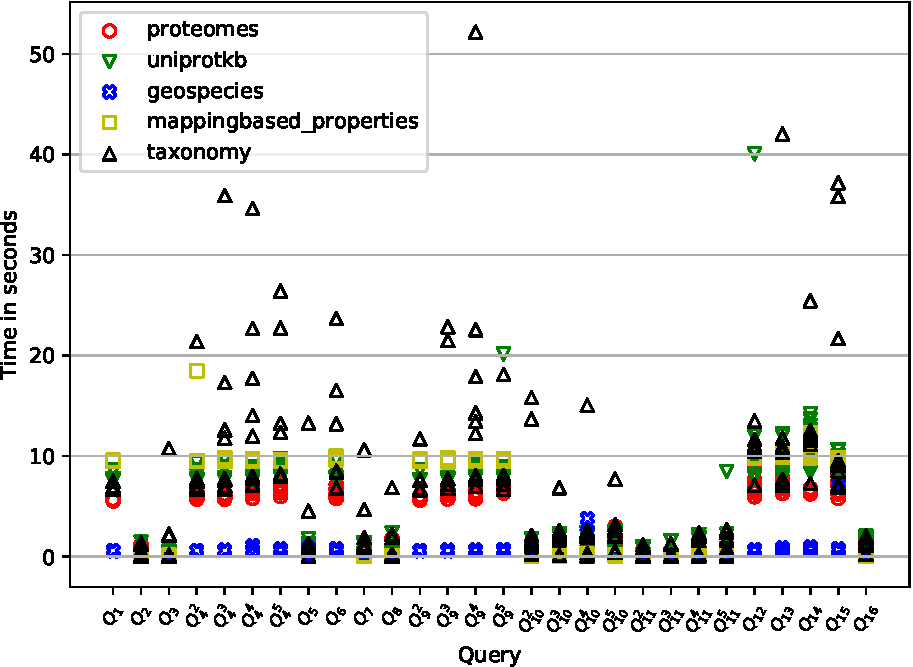
\includegraphics[width=0.48\textwidth]{data/other_all.pdf}
   \caption{Reachability index creation time for real-world RDFs}
   \label{fig:other_all_qs}
\end{figure}

Paths extraction was evaluated on cases with possible long paths.
These cases were selected during reachability index creation by using number of iterations in transitive closure evaluation.
For each selected graph and query we measure paths extraction time for each reachable pair, reachability index creation time is not included because exactly the same index, as calculated at the previous step, is used for paths extraction. 

We evaluate two scenarios.
The first one is a single path extraction.
In this case results are represented as a dependency of extraction time on extracted path length.
We can see linear !!!!

The second scenario is many paths extraction.
Here we limit a number of path to extract by !!! 
In this case results are represented as a dependency of extraction time on number of extracted paths.


\begin{figure}
     \begin{subfigure}[b]{0.24\textwidth}
         \centering
         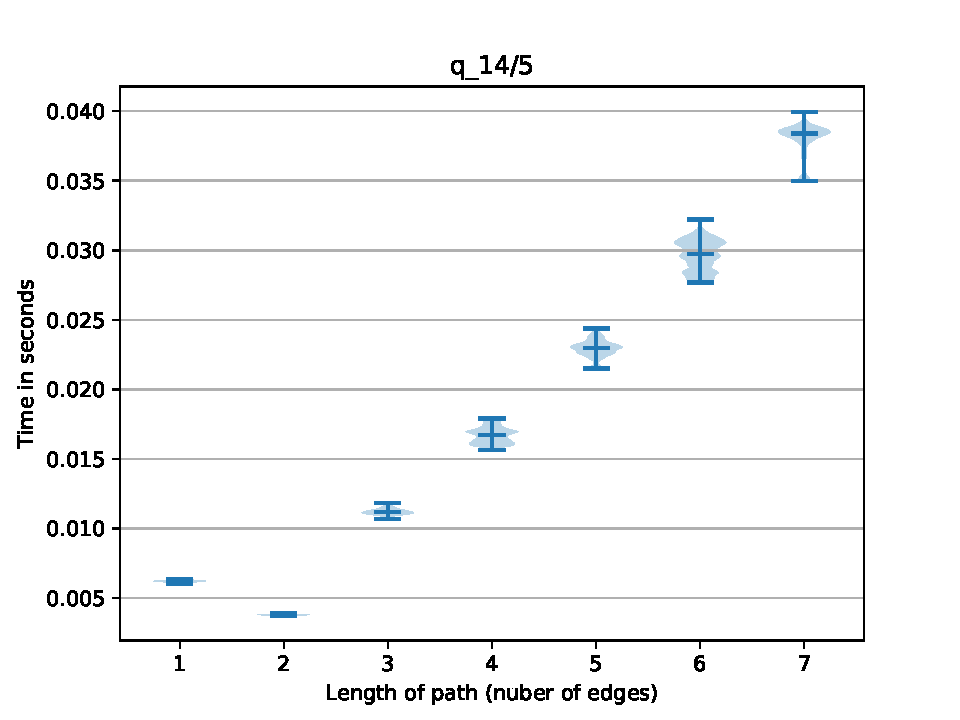
\includegraphics[width=\textwidth]{data/res_graphics/q_14_5.pdf}
         \caption{$y=x$}
         \label{fig:y equals x}
     \end{subfigure}
     ~\begin{subfigure}[b]{0.24\textwidth}
         \centering
         %\includegraphics[width=\textwidth]{data/res_graphics/q9_2_8.pdf}
         \caption{$y=x$}
         \label{fig:y equals x}
     \end{subfigure}\\
     \begin{subfigure}[b]{0.24\textwidth}
         \centering
         %\includegraphics[width=\textwidth]{data/res_graphics/q_14_8.pdf}
         \caption{$y=x$}
         \label{fig:y equals x}
     \end{subfigure}
     ~\begin{subfigure}[b]{0.24\textwidth}
         \centering
         %\includegraphics[width=\textwidth]{data/res_graphics/q4_2_8.pdf}
         \caption{$y=x$}
         \label{fig:y equals x}
     \end{subfigure}
   %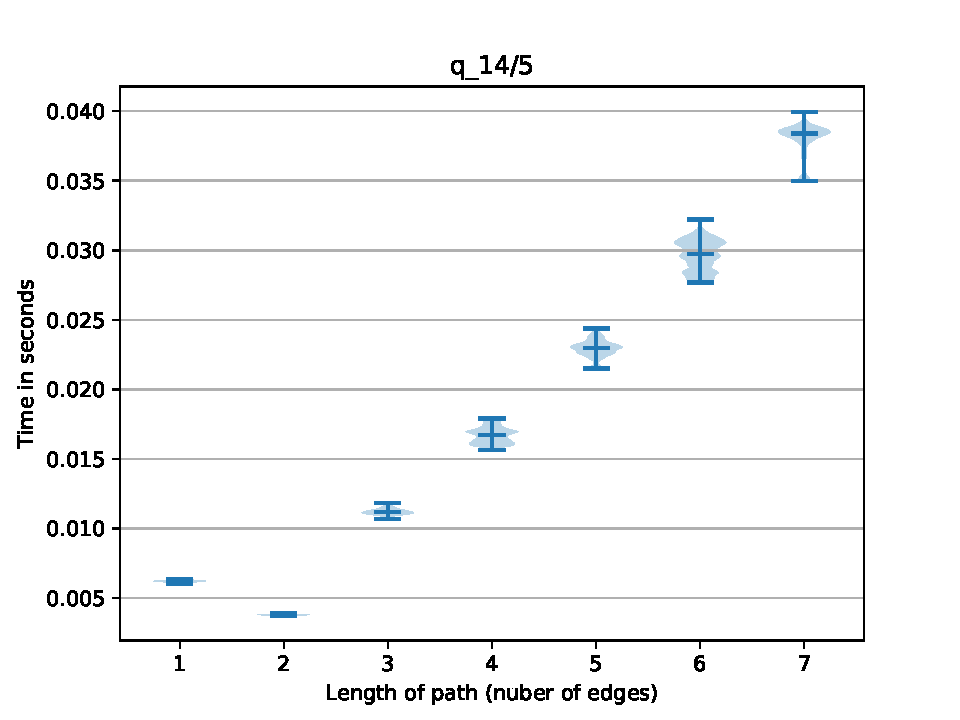
\includegraphics[width=0.48\textwidth]{data/res_graphics/q_14_5.pdf}
   \caption{Single path extraction}
\end{figure}

\subsubsection{Conclusion}

We can conclude that proposed algorithm is applicable for real-world data processing: the algorithm allows one both to solve reachability problem and to extract paths of interest in reasonable time even using na{\"i}ve implementation.  

\subsection{CFPQ Evaluation}

Comparison with matrix-based algorithm.

\subsubsection{Dataset}

Dataset for evaluation. 
It should be CFPQ\_Data\footnote{CFPQ\_Data is a dataset for CFPQ evaluation which contains both synthetic and real-world data and queries \url{https://github.com/JetBrains-Research/CFPQ\_Data}. Access date: 07.07.2020.}

\begin{table}
{
\rowcolors{2}{black!2}{black!10}
\begin{tabular}{|l|c|c|}
\hline
Graph & \#V & \#E \\
\hline
\hline 
eclass\_514en  & 120 926 & 484 646 \\
enzyme  & 358 434 & 144 9711 \\
geospecies  & 596 760 & 2 416 513 \\
go   & 1 188 340 & 4 820 728 \\
go-hierarchy & 1 780 956 & 7 228 358 \\
taxonomy & 2 308 385 & 9 369 511 \\
\hline
Aliases 1 & 6 442 630 & 24 465 430 \\
Aliases 2 & 4 834 262 & 12 366 973 \\
.... & 5 728 398 & 14 922 125 \\
\hline
\end{tabular}
}
\caption{Graphs for CFPQ evaluation}
\label{tbl:graphs_for_cfpq}
\end{table}



Same-generation queries, memory aliases.

\subsubsection{Results}

Results of evaluation.

Index creation.

{\setlength{\tabcolsep}{0.4em}
	\begin{table}
		\caption{RDFs query $G_1$ and $G_2$ (time is measured in seconds and memory is measured in megabytes)}
		\label{tbl:tableRDFQ1_appendix}
		\rowcolors{4}{black!2}{black!10}
		\small
		\begin{tabular}{| l | c | c | c | c |}
			\hline
			
			\multirow{2}{*}{Name}  & \multicolumn{2}{c|}{$G_1$} & \multicolumn{2}{c|}{$G_2$} \\
			\cline{2-5}
			                       & Tensors & RG\_CPU\textsubscript{path} & Tensors & RG\_CPU\textsubscript{path}	 \\
			\hline
			\hline
			eclass\_514en   & 0.254   & 0.195   & 0.227 & ...\\
			enzyme          & 0.035   & 0.029   & 0.036 & ...\\
			geospecies      & 0.091   & ...     & 0.001 & ...\\
			go-hierarchy    & 0.186   & 0.976   & 0.293 & ...\\
			go              & 1.676   & 1.286   & 1.368 & ...\\
			pathways        & 0.015   & 0.021   & 0.009 & ...\\
			taxonomy        & 5.366   & .....   & 3.282 & ...\\
			\hline
		\end{tabular}
	\end{table}
}


Paths extraction.

\subsubsection{Conclusion}

\section{Conclusion and future work}
In this paper, we shown how the context-free path query evaluation w.r.t. the relational and the single-path query semantics can be reduced to the calculation of matrix transitive closure. Also, we provided a formal proof of the correctness of the proposed reduction. In addition, we introduced an algorithm for computing this transitive closure, which allows us to efficiently apply GPGPU computing techniques. Finally, we shown the practical applicability of the proposed algorithm by running different implementations of our algorithm on real-world data.

We can identify several open problems for further research. In this paper we have considered only two semantics of context-free path querying but there are other important semantics, such as all-path query semantics~\cite{hellingsPathQuerying} which requires to present all paths for all triples $(A,m,n)$. Context-free path querying implemented with algorithm~\cite{GLL} can answer the queries in all-path query semantics by constructing a parse forest. It is possible to construct a parse forest for a linear input by matrix multiplication~\cite{okhotin_cyk}. Whether it is possible to generalize this approach for a graph input is an open question.

In our algorithm, we calculate the matrix transitive closure naively, but there are algorithms for the transitive closure calculation, which are asymptotically more efficient. Therefore, the question is whether it is possible to apply these algorithms for the matrix transitive closure calculation to the problem of context-free path querying.

Also, there are Boolean grammars~\cite{okhotinBoolean}, which have more expressive power than context-free grammars. Boolean path querying is an undecidable problem~\cite{hellingsRelational} but our algorithm can be trivially generalized to work on boolean grammars because parsing with boolean grammars can be expressed by matrix multiplication~\cite{okhotin_cyk}. It is not clear what a result of our algorithm applied to Boolean grammars would look like. Our hypothesis is that it would produce the upper approximation of a solution.

From a practical point of view, matrix multiplication in the main loop of the proposed algorithm may be performed on different GPGPU independently. It can help to utilize the power of multi-GPU systems and increase the performance of context-free path querying.

There is an algorithm~\cite{apspGPU} for transitive closure calculation on directed graphs which generalized to handle graph sizes inherently larger then the DRAM memory available on the GPU. Therefore, the question is whether it is possible to apply this approach to the matrix transitive closure calculation in the problem of context-free path querying.

\begin{acks}
The reported study was funded by RFBR, project number 19-37-90101.
\end{acks}

%
% The next two lines define the bibliography style to be used, and the bibliography file.
\bibliographystyle{ACM-Reference-Format}
\bibliography{cfpq_for_redisgraph}

%
% If your work has an appendix, this is the place to put it.
%\vspace{10cm}

%\appendix

%\section{Dataset description}\label{section:dataset}

In our evaluation we use dataset which contains the following parts.
{\setlength{\tabcolsep}{0.4em}
	\begin{table}[h]
		\caption{RDFs properties}
		\label{tbl:propRDF}
		\rowcolors{2}{}{lightgray}
		\begin{tabular}{| l | c | c | c | c |}
			\hline
			Name                  & \#V    & \#E     & \#type &\#subClassOf \\
			\hline
			\hline
			atom-primitive				& 291		& 685		& 138	& 122	\\
			univ-bench					& 179		& 413		& 84		& 36		\\
			travel						& 131		& 397		& 90		& 30		\\
			skos							& 144		& 323		& 70		& 1		\\
			people\_pets					& 337		& 834		& 161	& 33		\\
			generations					& 129		& 351		& 78		& 0		\\
			foaf							& 256		& 815		& 174	& 10		\\
			biomed-mesure-prim   	    & 341		& 711		& 130	& 122	\\
			funding						& 778		& 1480		& 304	& 90               \\
			pizza						& 671		& 2604		& 365	& 259              \\
			wine							& 733		& 2450		& 485	& 126              \\
			core							& 1323		& 8684		& 1412	& 178              \\
			pathways						& 6238		& 37196		& 3118 	& 3117             \\
			go-hierarchy					& 45007		& 1960436	& 0		& 490109           \\
			enzyme						& 48815		& 219390		& 14989	& 8163             \\
			eclass\_514en				& 239111		& 1047454	& 72517	& 90962            \\
			go							& 272770		& 1068622	& 58483	& 90512            \\
			\hline
		\end{tabular}
	\end{table}
}

{\setlength{\tabcolsep}{0.4em}
\begin{table*}[h]
\caption{RDFs query $G_2$ (time is measured in seconds and memory is measured in megabytes)}
\label{tbl:tableRDFQ2}
\rowcolors{3}{}{lightgray}
\begin{tabular}{| l | r  r | r  r | r  r | r  r | r  r |}
    \hline

    \multirow{3}{*}{Name}   &   \multicolumn{6}{|c|}{Relational semantics index}	&	\multicolumn{4}{|c|}{Single path semantics index} \\
    \cline{2-11}
    &	\multicolumn{2}{|c|}{RG\_CPU\textsubscript{rel}}	&	\multicolumn{2}{|c|}{RG\_CUSP\textsubscript{rel}}	&	\multicolumn{2}{|c|}{RG\_SPARSE\textsubscript{rel}} &	\multicolumn{2}{|c|}{RG\_CPU\textsubscript{path}}	&	\multicolumn{2}{|c|}{RG\_SPARSE\textsubscript{path}}	 \\
    \cline{2-11}
    &   Time & Mem &  Time     & Mem & Time     & Mem  &  Time     & Mem & Time     & Mem \\
    \hline
    \hline
    atom-primitive          & 0.001 & 0.3  & 0.001 & 0.1 & 0.002 & 0.1   & 0.001 & 0.3  & 0.002 & 0.1   \\
biomedical-mesure-primitive & 0.002 & 0.1  & 0.014 & 2.0   & 0.009 & 0.1   & 0.006 & 0.1  & 0.012 & 0.1   \\
core                        & 0.001 & 0.3  & 0.006 & 0.1 & 0.004 & 0.1   & 0.003 & 0.3  & 0.005 & 0.1   \\
eclass\_514en               & 0.035 & 6.5  & 0.020 & 16.0  & 0.100   & 12.0    & 0.123 & 17.7 & 0.127 & 18.0    \\
enzyme                      & 0.006 & 3.9  & 0.006 & 0.6 & 0.010  & 0.1   & 0.012 & 5.3  & 0.008 & 0.4   \\
foaf                        & 0.001 & 0.1  & 0.004 & 0.1 & 0.002 & 0.1   & 0.001 & 0.1  & 0.003 & 0.1   \\
funding                     & 0.002 & 0.1  & 0.015 & 0.4 & 0.007 & 0.1   & 0.009 & 0.1  & 0.008 & 0.1   \\
generations                 & 0.001 & 0.1  & 0.001 & 0.1 & 0.001 & 0.1   & 0.001 & 0.1  & 0.001 & 0.1   \\
go-hierarchy                & 0.095 & 17.8 & 0.253 & 528.0 & 0.175 & 130.4 & 0.884 & 88.8 & 0.306 & 138.8 \\
go                          & 0.306 & 25.8 & 0.240 & 84.0  & 0.181 & 25.4  & 0.918 & 78.1 & 0.219 & 34.2  \\
pathways                    & 0.005 & 0.2  & 0.005 & 0.4 & 0.004 & 0.1   & 0.017 & 0.5  & 0.003 & 0.1   \\
people\_pets                & 0.001 & 0.1  & 0.007 & 0.1 & 0.004 & 0.1   & 0.001 & 0.1  & 0.005 & 0.1   \\
pizza                       & 0.002 & 0.3  & 0.012 & 0.2 & 0.008 & 0.1   & 0.010  & 0.3  & 0.009 & 0.1   \\
skos                        & 0.001 & 0.1  & 0.001 & 0.1 & 0.001 & 0.1   & 0.001 & 0.1  & 0.002 & 0.1   \\
travel                      & 0.001 & 0.1  & 0.007 & 0.1 & 0.005 & 0.1   & 0.001 & 0.1  & 0.005 & 0.1   \\
univ-bench                  & 0.001 & 0.1  & 0.007 & 0.1 & 0.005 & 0.1   & 0.001 & 0.1  & 0.005 & 0.1   \\
wine                        & 0.001 & 0.3  & 0.006 & 0.1 & 0.004 & 0.1   & 0.002 & 0.3  & 0.004 & 0.1  \\
    \hline
  \end{tabular}
\end{table*}
}

\begin{itemize}
\item The real-world data RDFs provided in CFPQ\_Data dataset\footnote{CFPQ\_Data dataset GitHub repository: \url{https://github.com/JetBrains-Research/CFPQ_Data}. Access date: 12.11.2019.} from~\cite{Mishin:2019:ECP:3327964.3328503}.
\item Geospecies (RDF which contains information about biological hierrarchy\footnote{The Geospecies RDF: \url{https://old.datahub.io/dataset/geospecies}. Access date: 12.11.2019.} and same-generation query over \textit{broaderTransitive} relation) is provided in~\cite{Kuijpers:2019:ESC:3335783.3335791} and integrated in our evaluation with CFPQ\_Data.
\item It was shown in~\cite{Mishin:2019:ECP:3327964.3328503} that matrix-based algorithm is performant enough to handle bigger RDFs than those used in the initial datasets, such as~\cite{RDF}.
So, we add several big RDFs to CFPQ\_Data and use them in our evaluation.
New RDFs: \textit{go-hierarchy, go, enzime, core, pathways} are from UniProt database\footnote{Protein sequences data base: \url{https://www.uniprot.org/}. RDFs with data are avalable here: \url{ftp://ftp.uniprot.org/pub/databases/uniprot/current_release/rdf}. Access date: 12.11.2019}, and \textit{eclass-514en} is from eClassOWL project\footnote{eClassOWL project: \url{http://www.heppnetz.de/projects/eclassowl/}. eclass-514en file is available here: \url{http://www.ebusiness-unibw.org/ontologies/eclass/5.1.4/eclass_514en.owl}. Access date: 12.11.2019.}.
\end{itemize}

The properties of the RDFs from the dataset are given in table \ref{tbl:propRDF}. 
Geospecies RDF contains 450609 vertices, 2311461 edges, and 20867 edges labeled by \textit{broaderTransitive}.
Note that while the number of edges labeled by \textit{broaderTransitive} is equal to provided in~\cite{Kuijpers:2019:ESC:3335783.3335791}, the total number of vertices and edges is bigger. It is because we naively convert each triple from RDF to edge in the graph, while J. Kuijpers et al. use special \textit{neosemantics}\footnote{Neosemantix is an RDF processing plugin for Neo4j. Web page: \url{https://neo4j.com/labs/nsmtx-rdf/}. Access date: 30.03.2020.} plugin which can, for example, handling multivalued properties accurately.  

The variants of the \textit{same-generation query}~\cite{FndDB} are used in almost all cases because it is an important example of real-world queries that are context-free but not regular.
So, variations of the same generation query are used in our evaluation.
All queries are added to the CFPQ\_Data dataset.

We use two queries over \textit{subClassOf} and \textit{type} relations.
The first query is the grammar $G_1$:
\[
 \begin{array}{lcl}
   s  \rightarrow \textit{subClassOf}^{\ -1} \ s \ \textit{subClassOf}   & \quad & s  \rightarrow \textit{type}^{\ -1} \ s \ \textit{type}     \\
   s  \rightarrow \textit{subClassOf}^{\ -1} \ \textit{subClassOf}       & \quad & s  \rightarrow  \textit{type}^{\ -1}  \ \textit{type}

 \end{array}
 \]
The second one is the grammar $G_2$: \[s \rightarrow \textit{subClassOf}^{\ -1} \ s \ \textit{subClassOf} \mid \textit{subClassOf}\]

For geospecies we use same-generation query \textit{geo} from the original paper~\cite{Kuijpers:2019:ESC:3335783.3335791}: \[s \rightarrow \textit{broaderTransitive} \ s \ \textit{broaderTransitive}^{\ -1} \]
\[s \rightarrow \textit{broaderTransitive}  \ \textit{broaderTransitive}^{\ -1} \]


\section{Evaluation Details}

Results for RDFs querying with $G_2$ grammar are presented in table~\ref{tbl:tableRDFQ2}.
We can see, that for small graphs time for both relational and single-path querying are similar for CPU and GPGPU versions, but for bigger graphs (\textit{go} and \textit{go-hierarchy}, for example) GPUPU version is more performant than CPU one.

\balance



%\subsection{Part One}


\end{document}
